\documentclass{report}
\usepackage[spanish]{babel}
\usepackage[utf8]{inputenc}
\usepackage{graphicx}

\title{{\bf Práctica 4:} Conversión de Expresión Regular a Automata Finito Determinista}

%%
%% Escriban el nombre de los colaboradores aquí
%%

\author{{\bf SAUCEDO DELGADO RAFAEL NORMAN} {- Líder del proyecto}
\and ACEVES AMADOR OMAR EMMANUEL
\and BARAJAS URIBE SERGIO
\and CHAVEZ RUEDAS DANIELA BERENICE
\and CRUZ UBALDO ERICK
\and FIGUEROA URBINA ERYK ALBERTO
\and GARCIA SOTO ELIAS ENRIQUE
\and GONZALEZ FLORES BYRON
\and GONZALEZ SOLIS ALEJANDRO
\and HERNANDEZ JIMENEZ ENRIQUE
\and HERNANDEZ MELGAREJO LUIS ANTONIO
\and LORENZO RUIZ MIGUEL ANGEL
\and MARTINEZ MARTINEZ SERGIO IVAN
\and MUÑOZ MENDOZA JESSICA LIZBETH
\and ORTEGA ROJAS HUGO
\and ROMERO GUTIERREZ MIGUEL ANGEL
\and SANCIPRIÁN LUCERO RUDY
\and TORRES RODRIGUEZ ESTEBAN ALBERTO
\and VAZQUEZ REYES JOSE LUIS
\and VIVANCO CARMONA ERICK RAFAEL
}

\begin{document}

\maketitle
\tableofcontents

\chapter{Análisis}


\section{Objetivo}
El programa deberá convertir una Expresión Regular (E.R.) a un Autómata Finito Determinista(A.F.D.).
Dicha tarea se programará apegándose al algoritmo <<del Árbol>>.


\section{Requerimientos Funcionales}
\begin{itemize}
	\item El programa recibirá como entrada una expresión regular la cual será transformada en un Automata Finito Determinista.
	\item Generará como salida una imagen del AFD.
\end{itemize}


\section{Requerimientos No Funcionales}
\begin{itemize}
	\item La aplicación debe ejecutarse en todo Sistema Operativo basado en UNIX.
	\item Se usará el paradigma orientado a objetos utilizando el lenguaje C++.
	\item La computadora en la cual se ejecutará la aplicación deberá tener instalado DOT.
\end{itemize}


\section{El algoritmo}
El programa que se realizará constará de la conversión de una Expresión Regular (E.R.) a un Autómata Finito Determinista (A.F.D.), dicha tarea se programará apegándose al algoritmo (del Árbol).
Los pasos del algoritmo se pueden listar como:
\begin{enumerate}
	\item Extender la E.R. que se va a convertir.
	\item Construir el árbol de análisis sintáctico correspondiente a la E.R.
	\item Anotar las posiciones de los símbolos que están en la E.R.
	\item Anotar en cada nodo si es anulable o no.
	\item Anotar en cada nodo las posiciones de la función primero().
	\item Anotar en cada nodo las posiciones de la función último().
	\item Llenar la tabla de las posiciones siguientes.
	\item Determintar los estados del A.F.D usando los siguientes.
	\item Marcar el estado inicial y los finales.
\end{enumerate}
La explicación de los puntos anteriores, de una forma más detallada, es la siguiente:

\begin{enumerate}
	\item Se extiende la E.R., de la siguiente forma: E.R.\#, donde \# es un marcador final que se añade a la E.R. y que difiere de los caracteres que pueden aparecer en E.R.
	\item Se construirá el árbol sintáctico para la E.R. a partir del análisis sintáctico de la misma; para ello sabemos que un árbol tiene 2 tipos de nodos: nodos hojas y nodos que no son hojas que aquí representarán operaciones. En un árbol sintáctico de una E.R. los nodos hojas representarán un carácter, el resto de los nodos representarán operaciones. Por esto, tendremos estos nodos posibles:
	\begin{itemize}
		\item Nodo Hoja: se representa con un círculo y dentro del mismo el caracter que hay en esa posición.
		\item Nodo concatenación: se representa con un círculo con un punto adentro.
		\item Nodo disyunción: se representa con un círculo con un | adentro.
		\item Nodo asterisco: se representa con un círculo y un * adentro.
		\item Nodo uno o más: se representa con un círculo y un + adentro.
	\end {itemize}
	\item Los nodos anulables se pueden calcular con ayuda de la siguiente tabla. Ver tabla \ref{fig:anulable}.

	\begin{figure}
		\centering
		%%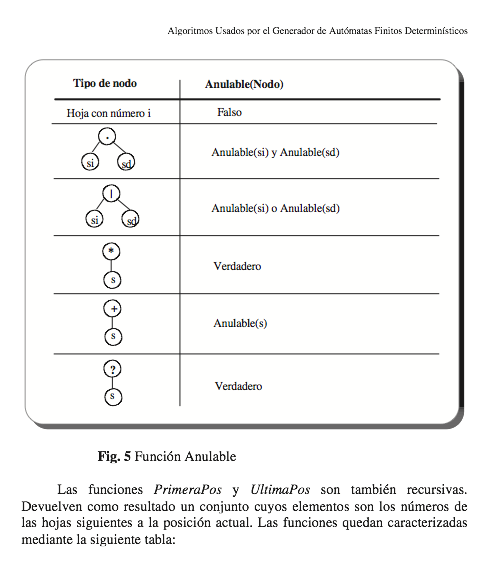
\includegraphics[width=12cm]{img/tabla1.png}
		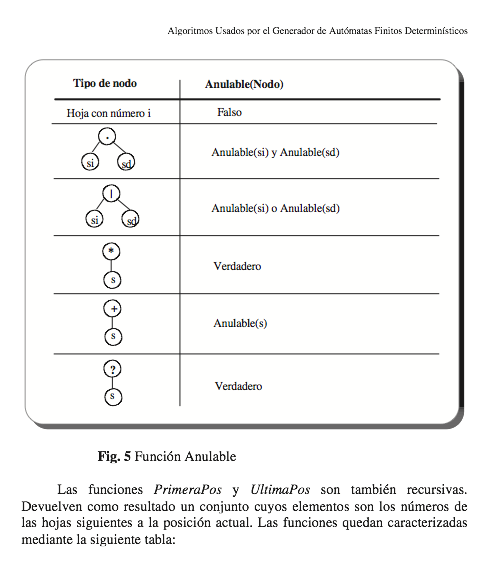
\includegraphics[scale=.5]{img/tabla1.png}
		\caption{Función anulable.}
		\label{fig:anulable}
	\end{figure}

	\item Para calcular los nodos primeros y últimos, se puede utilizar la siguiente tabla. Ver tabla \ref{fig:primeros y ultimos}.

	\begin{figure}
		\centering
		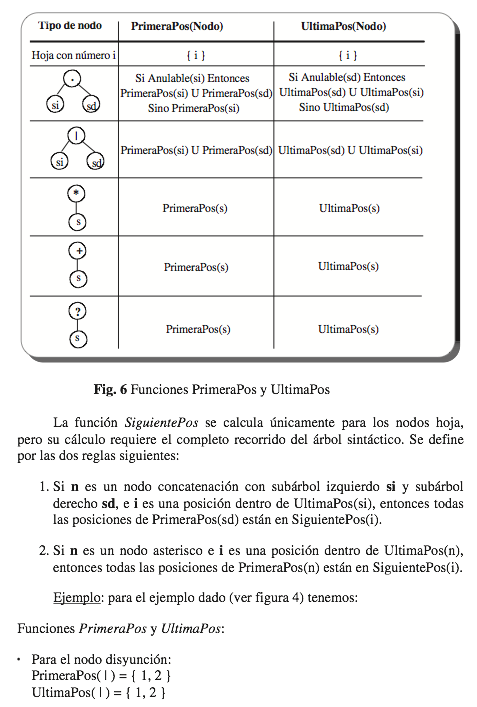
\includegraphics[scale=0.5]{img/tabla2.png}
		\caption{Funciones Primera Posición y Última Posición.}
		\label{fig:primeros y ultimos}
	\end{figure}

	\item Para calcular los siguientes, solo se utilizan los nodos hojas, pero su cálculo requiere el completo recorrido del árbol sintáctico. Se define por las dos reglas siguientes:

	\begin{itemize}
		\item Si {\bf n} es un nodo concatenación con subárbol izquierdo {\bf si} y subárbol derecho {\bf sd}, e {\bf i} es una posición dentro de los últimos, entonces todas las posiciones de primeros están en siguientes.
		\item Si  {\bf n} es un nodo asterisco e {\bf i} es una posición dentro de últimos, entonces todas las posiciones de primeros están en siguiente.
	\end{itemize}

	\item Calcular los estados del A.F.D., al principio, cada estado está “no marcado”, y un estado se convierte en “marcado” justo antes de considerar sus transiciones de salida. El estado inicial del A.F.D., son los primeros de la raíz, y los estados de aceptación son todos los que contienen la posición asociada con el marcador \#. El procedimiento de cálculo del conjunto de estados y de la tabla de transiciones del A.F.D. para la E.R. es el que se muestra en el siguiente algoritmo. Ver figura \ref{fig:algoritmo}.

	\begin{figure}
		\centering
		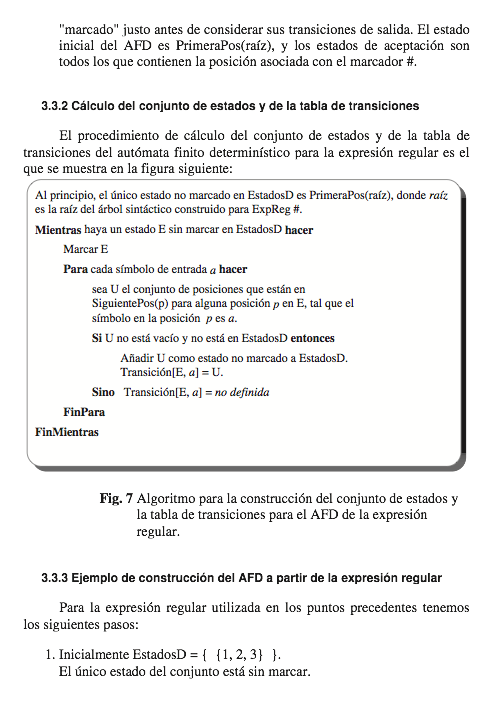
\includegraphics[scale=.5]{img/tabla3.png}
		\caption{Algoritmo para la construción del conjunto de estados y la tabla de transiciones para el AFD de la expresión regular.}
		\label{fig:algoritmo}
	\end{figure}

\end{enumerate}

\section{Ejemplo}
%Presentar un ejemplo con la expresión regular (a|b+)c* que contiene todos los operadores.





\chapter{Diseño}


\chapter{Implementación}


\chapter{Pruebas}


\chapter{Anexos}








\end{document}
